\documentclass[
    12pt,
    a4paper,
    oneside
]{article}

% -------------------------------------------------
% PACOTES
% -------------------------------------------------

\usepackage[brazil]{babel}
\usepackage[utf8]{inputenc}
\usepackage[T1]{fontenc}

\usepackage{times}
\usepackage{indentfirst}
\usepackage{graphicx}
\usepackage{float}
\usepackage{xcolor}
\usepackage{amsmath}
\usepackage{setspace}
\usepackage{geometry}
\usepackage{titlesec}
\usepackage{caption}

\usepackage{listings}
\usepackage{tabularx}
\usepackage{float}
% -------------------------------------------------
% CONFIGURAÇÕES ABNT
% -------------------------------------------------

\geometry{
    a4paper,
    left=3cm,
    right=2cm,
    top=3cm,
    bottom=2cm
}

\setlength{\parindent}{1.25cm}
\setlength{\parskip}{0cm}

\onehalfspacing

% -------------------------------------------------
% INÍCIO DO DOCUMENTO
% -------------------------------------------------

\begin{document}

% -------------------------------------------------
% CAPA
% -------------------------------------------------

\begin{titlepage}

    \begin{minipage}[c]{0.3\textwidth}
        \raggedright
        \raisebox{0pt}[\height][0pt]{%
            
\includegraphics[width=4cm]{imagens/Logo_UnB.png}%
        }
    \end{minipage}
    \hfill
    \begin{minipage}[c]{0.7\textwidth}
        \centering
        \textbf{\LARGE Universidade de Brasília}\\[0.25cm]
        \textbf{\large Departamento de Ciência da Computação}\\[0.1cm]
    \end{minipage}

    \begin{center}
        \vspace{4cm}

        {\Large \textbf{Teleinformática e Redes 2}}

        \vspace{1cm}

        {\large Política 2: Análise de Deficiências + Política 2 + Failover}

        \vfill

        \textbf{Membros}

        \vspace{0.5cm}

        Daniel Lincoln Lopes de Souza -- 202042829\\
        Isabela Soares Furlan -- 231013636\\
        Luiz Fernando Candido Soaris -- 190092025

        \vfill

        Brasília -- DF\\
        \today

    \end{center}

\end{titlepage}

% -------------------------------------------------
% SUMÁRIO
% -------------------------------------------------

\tableofcontents
\newpage

% -------------------------------------------------
% INTRODUÇÃO
% -------------------------------------------------

\section{Introdução}

% Escreva aqui

% -------------------------------------------------
% DESENVOLVIMENTO
% -------------------------------------------------

\section{Análise de Deficiências}

\subsection{Evidências Coletadas}

A análise foi feita a partir dos arquivos CSV gerados pela Política 1. O arquivo \\ \texttt{metrics\_20260608\_220922.csv}\\
foi usado como principal trace de referência, pois representa um cenário sem rebuffering, mas com baixa utilização da vazão disponível. Nesse CSV, a vazão média medida foi de 696,54 kbps, enquanto o bitrate médio selecionado foi de apenas 340,00 kbps. Assim, o baseline utilizou aproximadamente 55,68\% da vazão disponível.

Alguns segmentos mostram essa deficiência de forma mais clara. No segmento 2, a vazão medida foi de 648,36 kbps, mas a qualidade selecionada permaneceu em 240p, com bitrate de 200 kbps, correspondendo a apenas 30,8\% da vazão medida. No segmento 3, a vazão foi de 722,93 kbps e o bitrate continuou em 200 kbps, apenas 27,7\% da vazão. Mesmo depois da subida para 360p, o cliente continuou conservador: no segmento 4, a vazão medida foi de 1004,17 kbps, mas o bitrate escolhido foi 400 kbps, isto é, 39,8\% da vazão.

\subsection{Oscilação de Qualidade}

Os dados não mostram uma oscilação severa de qualidade. No trace principal, a Política 1 realizou apenas uma troca de qualidade: começou em 240p e subiu para 360p. Portanto, a oscilação de qualidade não foi considerada a principal deficiência do baseline.

\subsection{Rebuffering}

No trace principal, não houve eventos de rebuffering. O CSV registra 0 eventos de rebuffering e 0,0 segundo de stall total. Isso indica que a Política 1 foi conservadora o suficiente para evitar interrupções de reprodução nesse cenário.

\subsection{Subutilização de Banda e Adaptação Conservadora}

A deficiência concreta identificada foi a subutilização da banda disponível. A Política 1 usa um fator de segurança fixo e ignora o nível do buffer no momento da decisão. Com isso, mesmo quando o buffer já estava suficiente para reprodução contínua, a política manteve qualidades baixas por vários segmentos. O resultado foi uma reprodução estável, mas com qualidade inferior ao que a rede e o buffer permitiam.


\section{Implementação da Política 2}
\subsection{Escolha da Política 2}

A Política 2 implementada foi uma política Buffer-Based ABR. Diferentemente da Política 1, que decide a qualidade com base diretamente na vazão média recente, a Política 2 usa o nível do buffer como principal sinal de decisão. A motivação é que um buffer alto indica maior margem para escolher uma qualidade superior sem aumentar imediatamente o risco de rebuffering.

A regra usada foi:

\begin{itemize}
    \item se o buffer for menor que 4 segundos, selecionar a menor qualidade;
    \item se o buffer estiver entre 4 e 8 segundos, selecionar a qualidade intermediária;
    \item se o buffer for maior ou igual a 8 segundos, selecionar a maior qualidade disponível.
\end{itemize}

No código, essa política foi implementada no script \texttt{policy\_comparison.py}. O mesmo script também executa a Política 1 sobre o mesmo trace de vazão, permitindo uma comparação controlada entre as duas políticas. Para manter a justiça da comparação, ambas as políticas foram avaliadas sobre a mesma sequência de vazões do CSV baseline \\ \texttt{metrics\_20260608\_220922.csv}.

\subsection{Comparação entre Políticas}

Para comparar as políticas sob o mesmo cenário de banda, foi usado um replay controlado do trace de vazão medido pela Política 1. A duração de segmento usada na simulação foi de 2 segundos, estimada a partir do nível inicial de buffer registrado no CSV.

\begin{table}[H]
\centering
\caption{Comparação entre Política 1 e Política 2 no mesmo trace de vazão}
\begin{tabular}{|l|c|c|}
\hline
\textbf{Métrica} & \textbf{Política 1} & \textbf{Política 2} \\
\hline
Vazão média medida & 696,54 kbps & 696,54 kbps \\
\hline
Bitrate médio selecionado & 340,00 kbps & 430,00 kbps \\
\hline
Utilização média da vazão & 55,68\% & 68,16\% \\
\hline
Trocas de qualidade & 1 & 2 \\
\hline
Eventos de rebuffering & 0 & 0 \\
\hline
Stall total & 0,0 s & 0,0 s \\
\hline
Buffer final & 11,52 s & 9,02 s \\
\hline
\end{tabular}
\end{table}

O resultado mostra que a Política 2 aumentou o bitrate médio de 340,00 kbps para 430,00 kbps, elevando a utilização média da vazão de 55,68\% para 68,16\%. Esse ganho foi obtido sem introduzir rebuffering no trace avaliado. O buffer final foi menor na Política 2, 9,02 s contra 11,52 s, o que é esperado, pois a política passou a consumir mais banda para entregar segmentos de maior qualidade.

\begin{figure}[H]
    \centering
    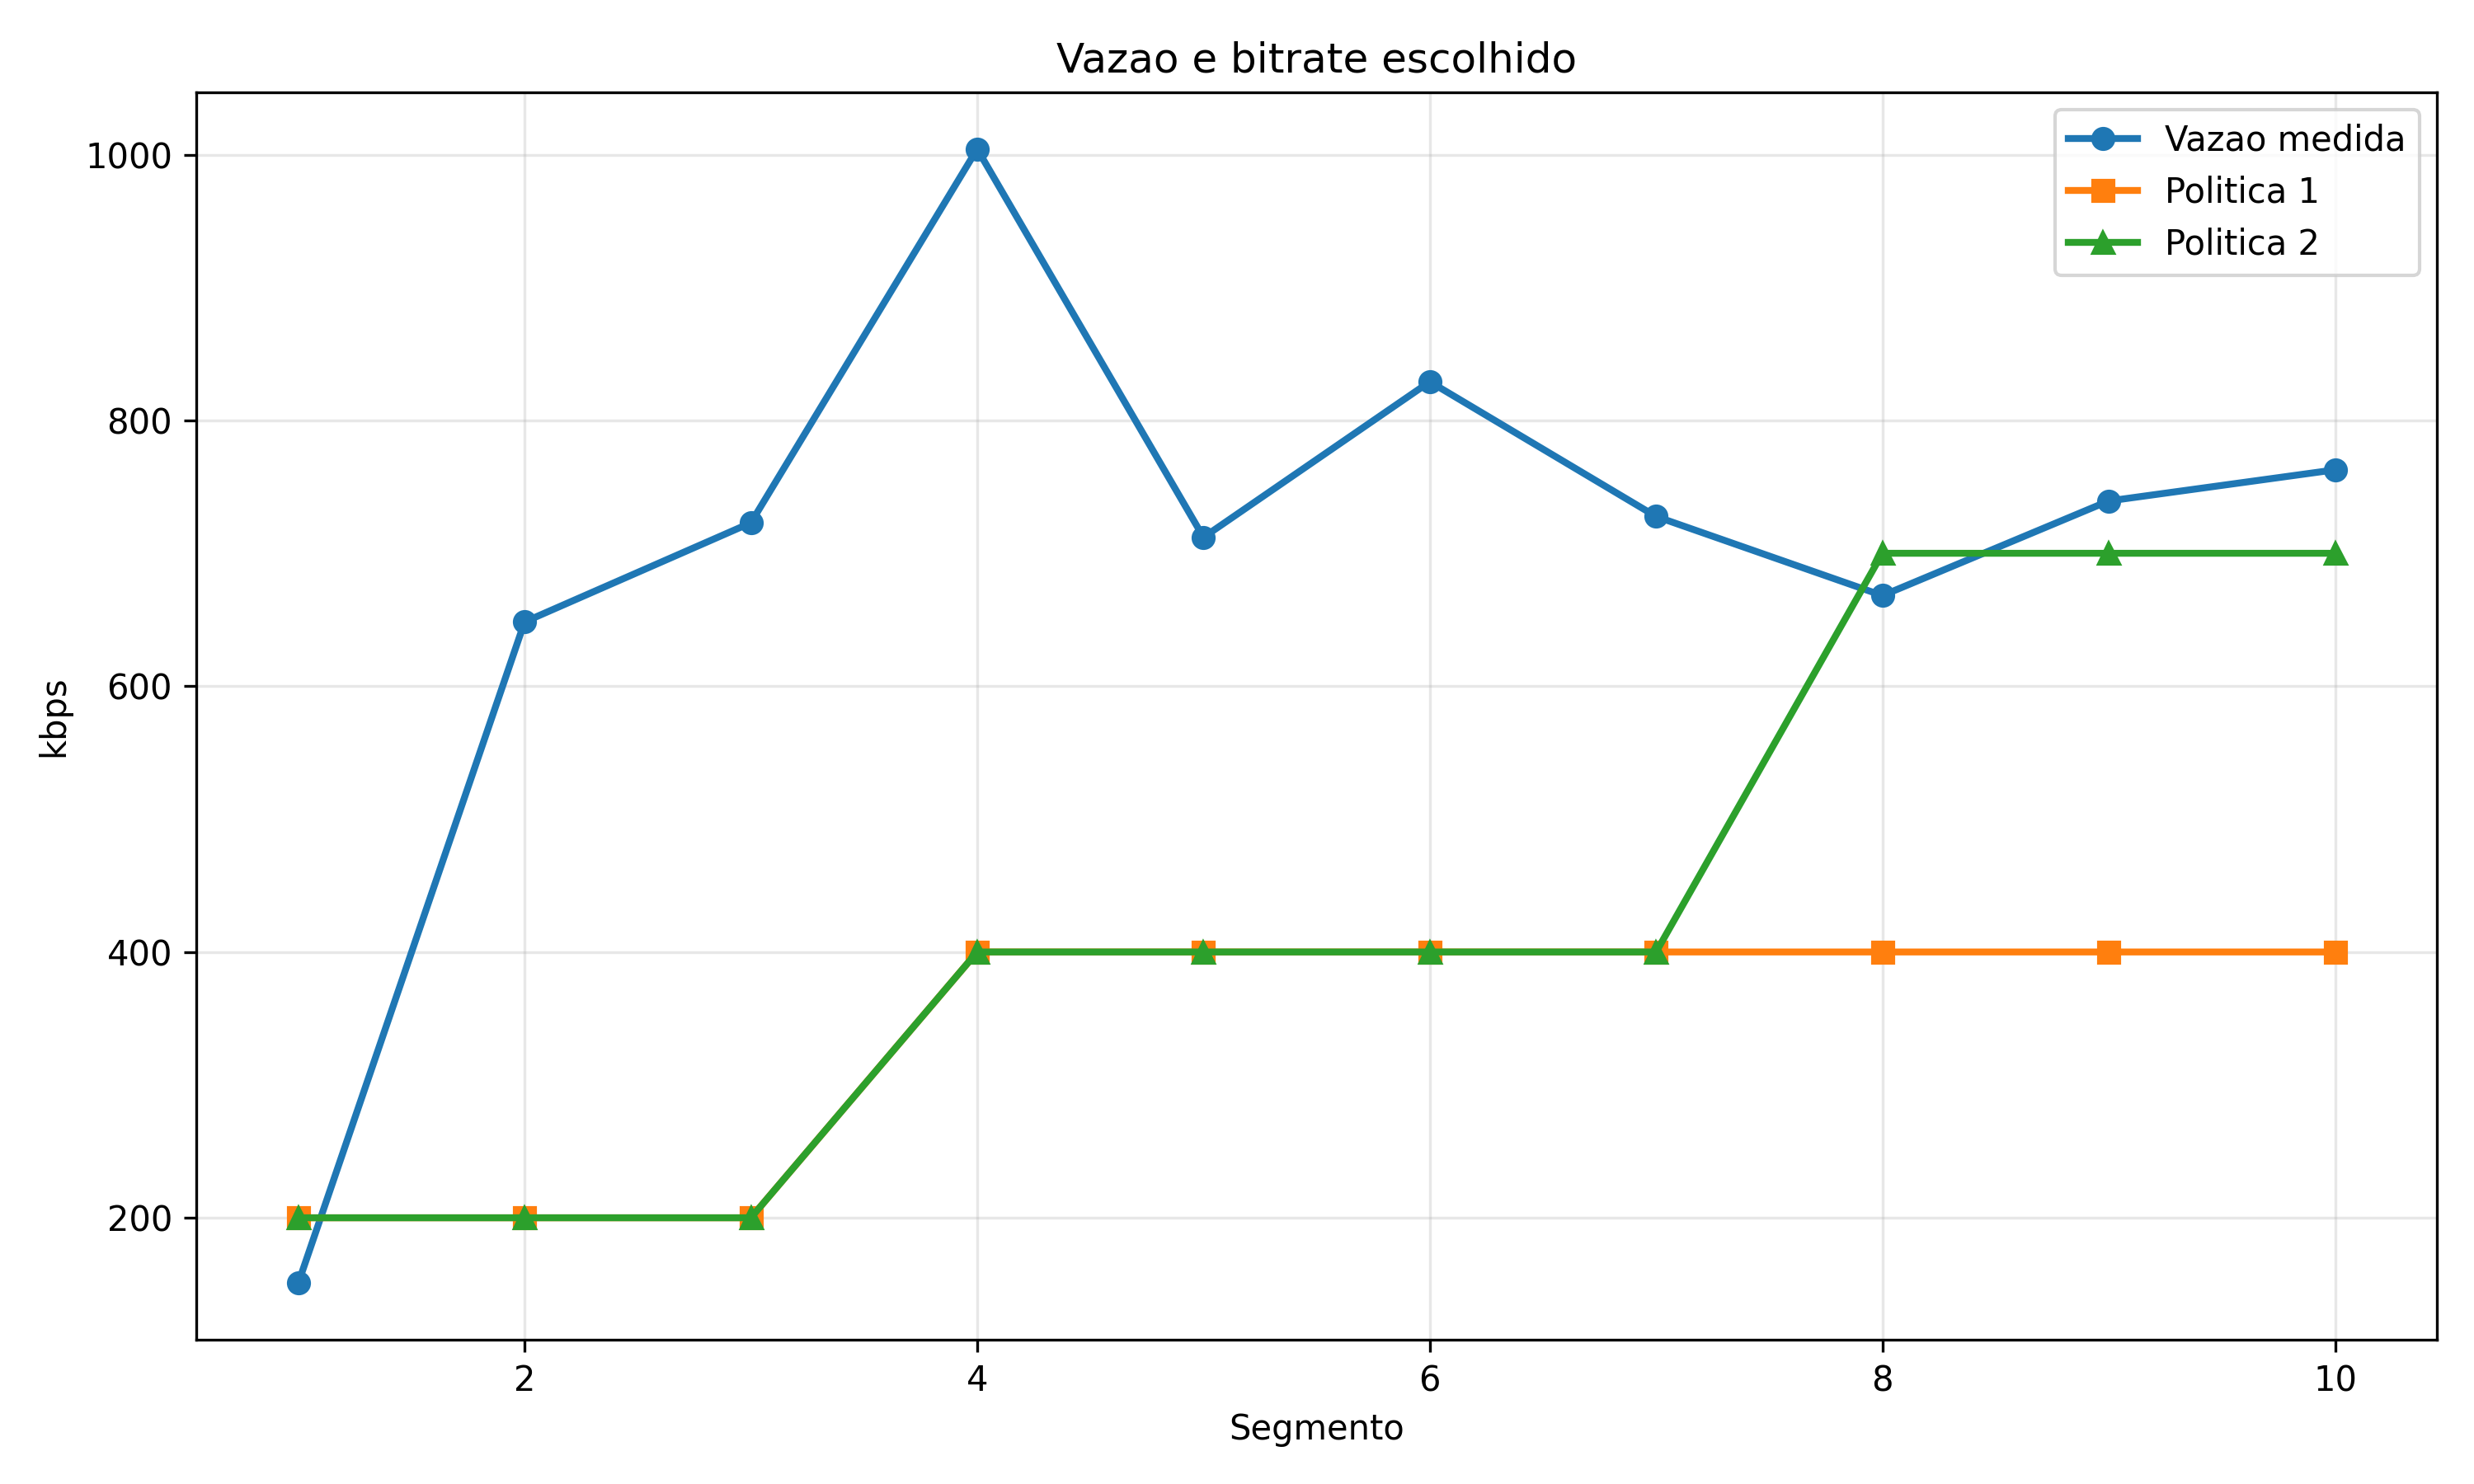
\includegraphics[width=0.95\textwidth]{plots/politica2_throughput_bitrate_overlay.png}
    \caption{Vazão medida e bitrate escolhido pelas duas políticas}
\end{figure}

\begin{figure}[H]
    \centering
    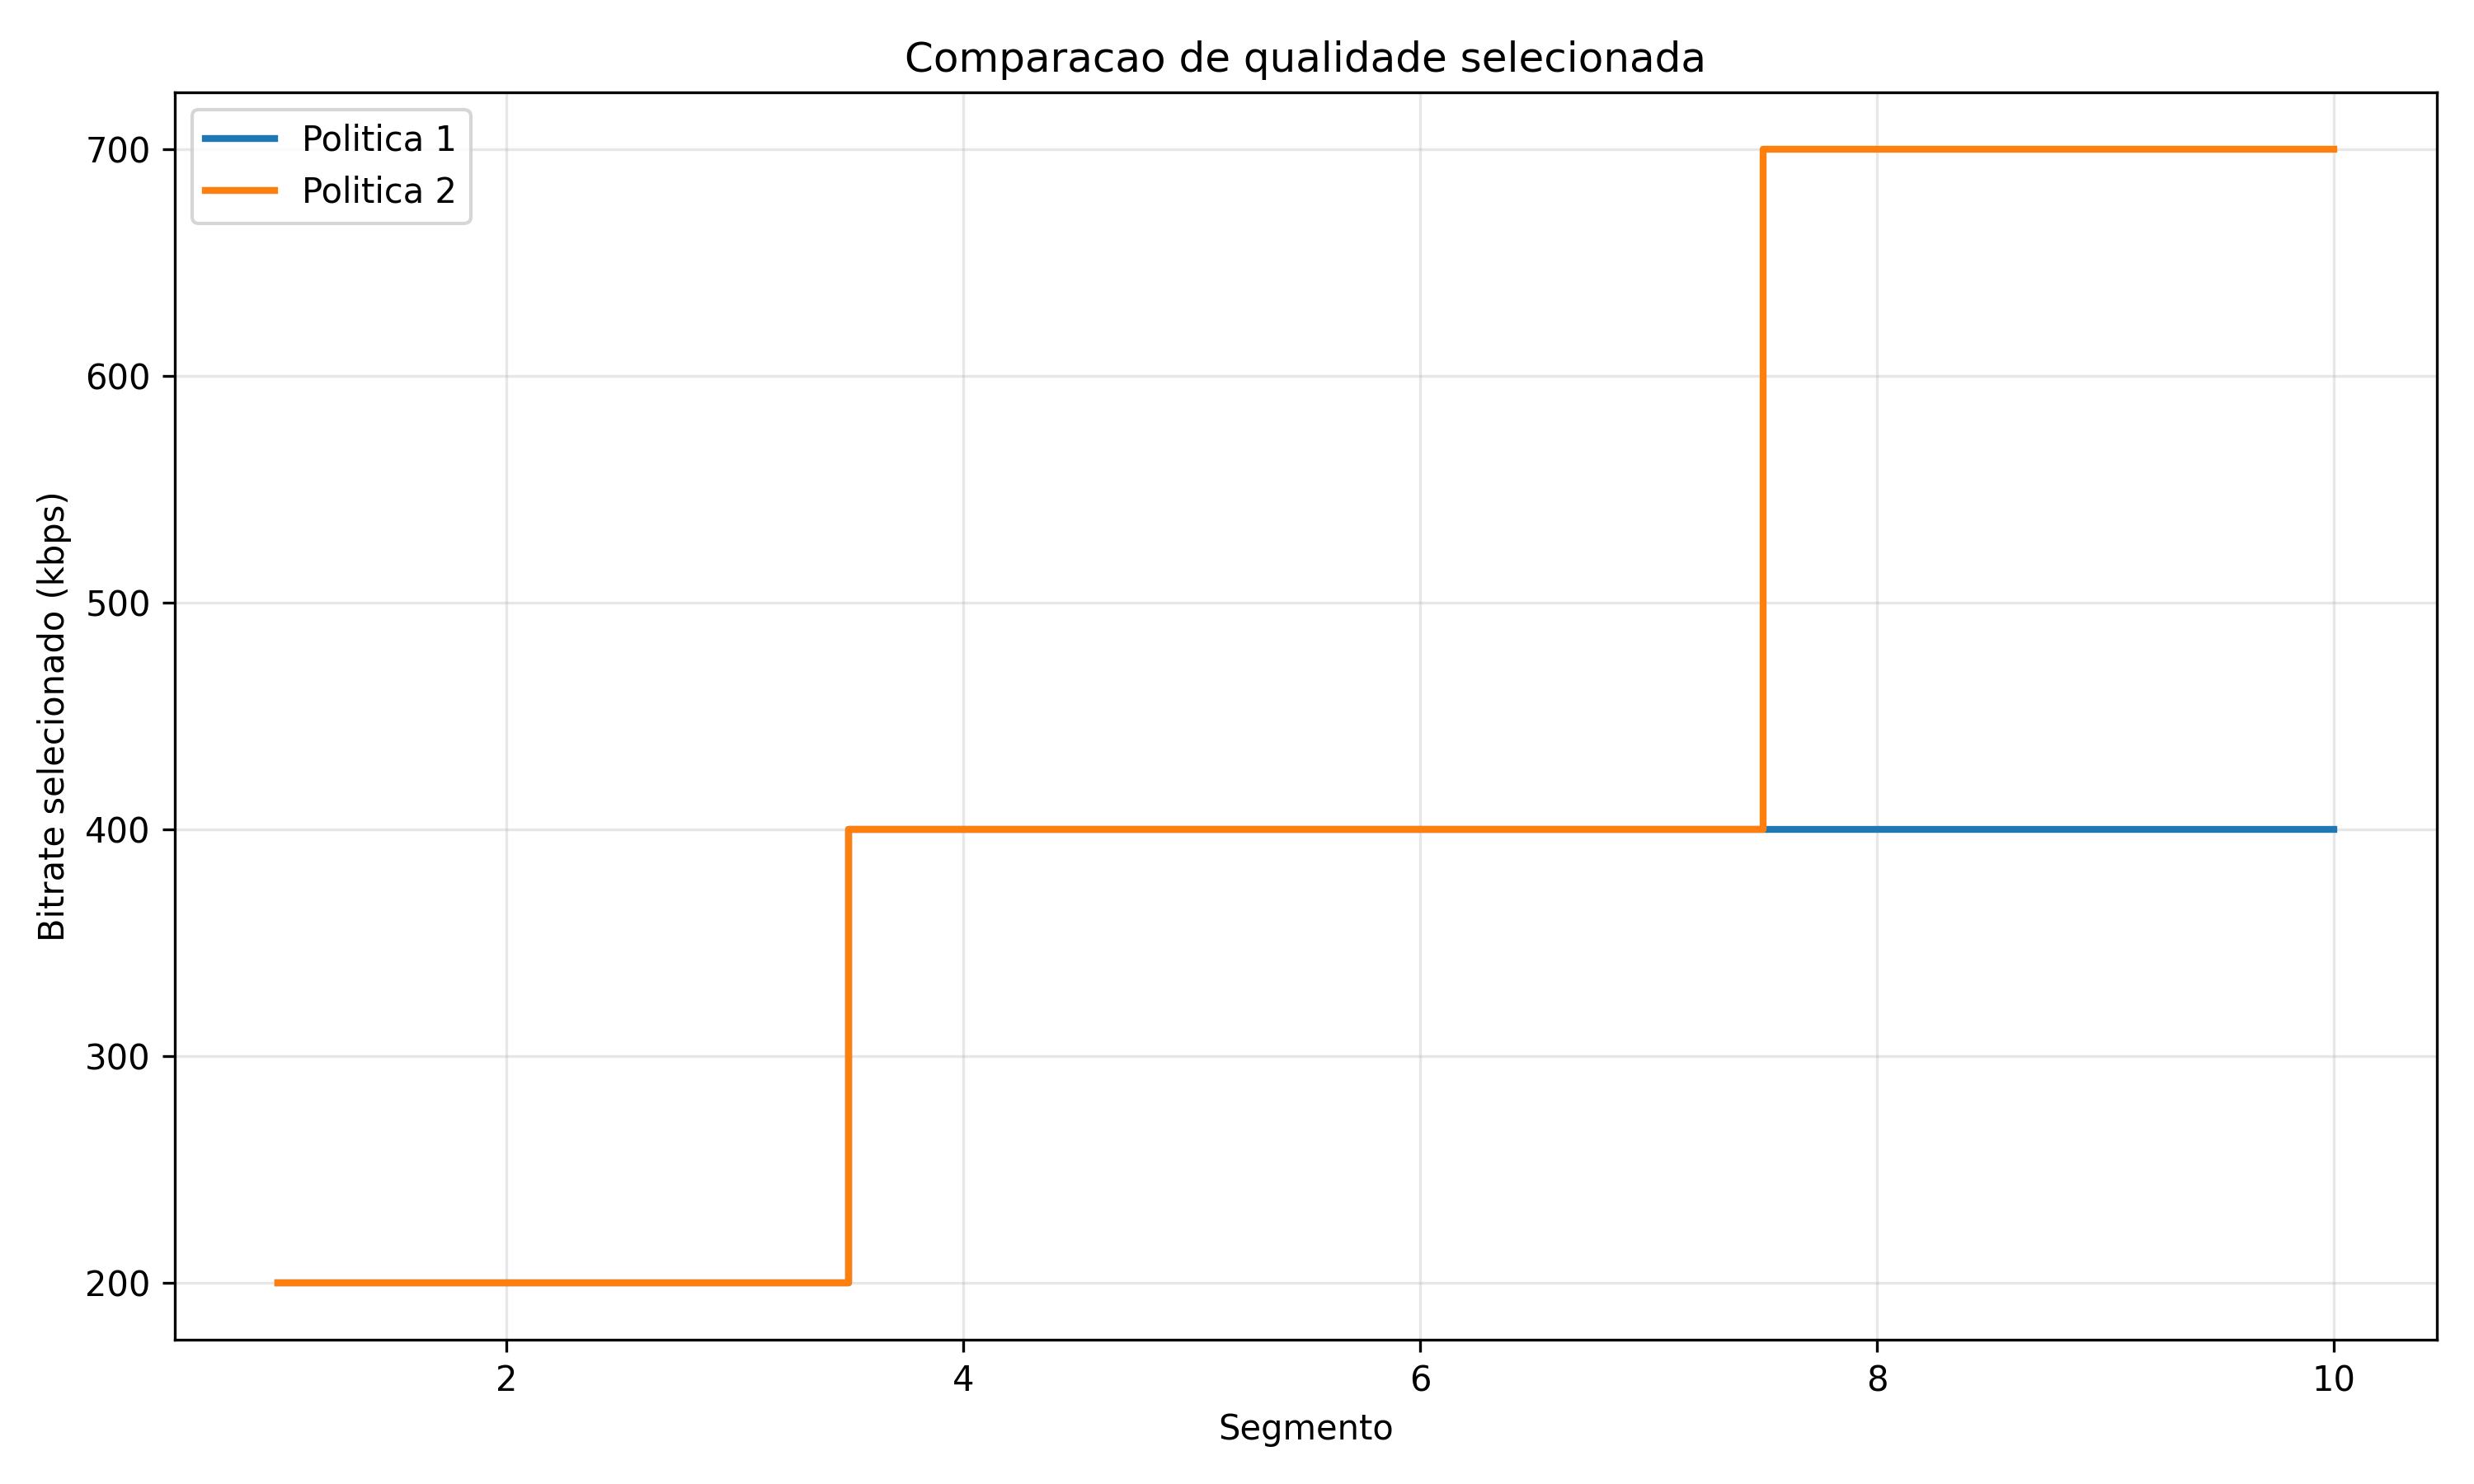
\includegraphics[width=0.95\textwidth]{plots/politica2_quality_comparison.png}
    \caption{Comparação da qualidade selecionada ao longo dos segmentos}
\end{figure}

\begin{figure}[H]
    \centering
    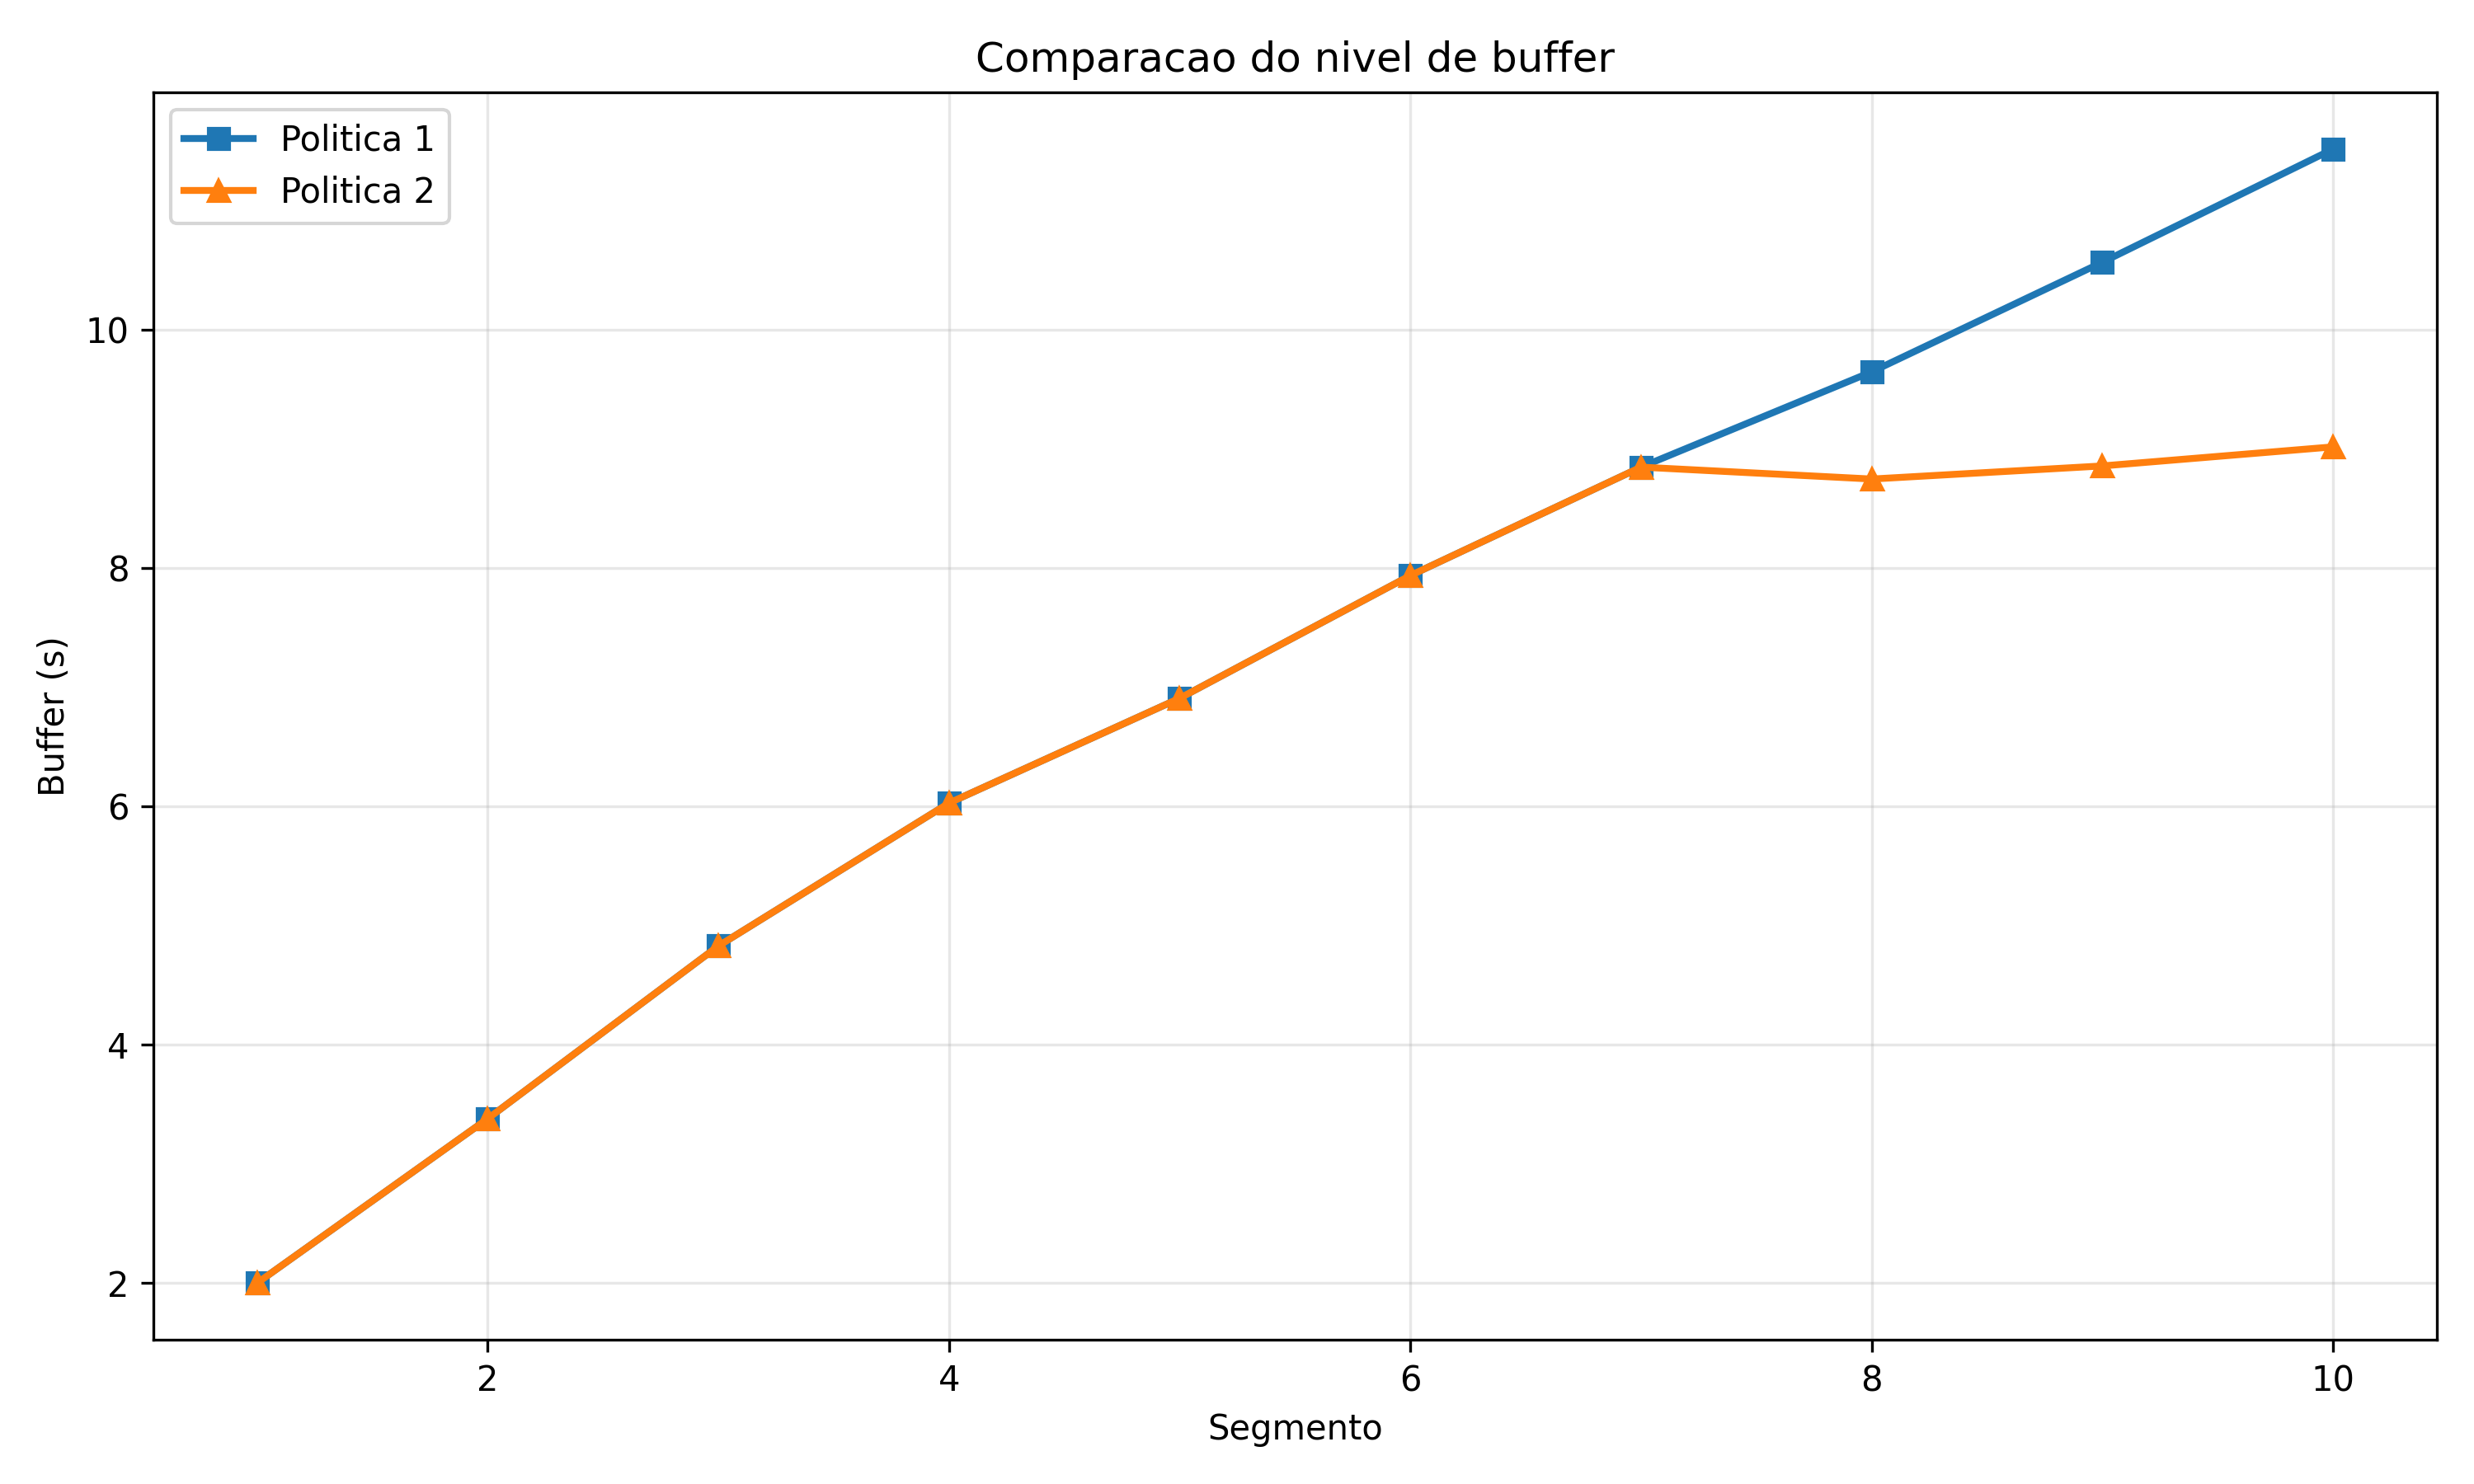
\includegraphics[width=0.95\textwidth]{plots/politica2_buffer_comparison.png}
    \caption{Comparação do nível de buffer ao longo dos segmentos}
\end{figure}

\section{Failover}

\subsection{Detecção de Falhas}

O cliente monitora falhas durante o download dos segmentos. Sempre que uma requisição HTTP gera uma exceção (\texttt{RequestException}), o segmento é considerado indisponível no servidor atual. Para fins de teste, também foram inseridas falhas forçadas em segmentos específicos, permitindo validar o comportamento do mecanismo de failover sob diferentes cenários.

\subsection{Seleção do Servidor de Backup}

A seleção do servidor de backup foi implementada na classe \texttt{ServerManager}. Os servidores são ordenados pela prioridade definida no manifest. Quando ocorre uma falha, o método \texttt{failover()} procura o próximo servidor disponível executando um \textit{health check} no endpoint \texttt{/health}. O primeiro servidor que responde corretamente é promovido a servidor ativo e passa a atender os downloads subsequentes.

\subsection{Continuidade da Reprodução}

Após a troca de servidor, o cliente reconstrói a URL do mesmo segmento e repete o download utilizando o novo servidor. Dessa forma, a recuperação ocorre de maneira transparente para a lógica de reprodução, sem perda do segmento solicitado.

O tempo necessário para realizar a troca é medido pela métrica \texttt{failover\_time}, calculada entre o início do processo de failover e a conclusão do download bem-sucedido no servidor substituto.

\subsection{Avaliação do Impacto no Buffer}

Para avaliar o efeito do failover na experiência do usuário, foi registrada a variável \texttt{buffer\_absorbed\_failover}. Essa métrica indica se o nível de buffer disponível foi suficiente para absorver o atraso introduzido pela troca de servidor.

Quando ocorre failover sem rebuffering, o evento é classificado como absorvido pelo buffer. Caso a troca provoque esgotamento do buffer e interrupção da reprodução, o failover é classificado como não absorvido. Essa distinção permite diferenciar falhas recuperadas de forma transparente daquelas que impactam diretamente a continuidade da reprodução.

% =====================================================================
% RESPOSTAS ÀS PERGUNTAS OBRIGATÓRIAS (Entrega 2)
% =====================================================================

\section{Respostas às Perguntas da Entrega 2}

\begingroup
\sloppy  % quebras de linha mais suaves

\begin{enumerate}
    \item \textbf{“Mostre no código onde o buffer é atualizado após cada segmento”}
    
    A atualização ocorre na classe \texttt{BufferManager} (arquivo \texttt{buffer\_manager.py}). Os métodos principais são:
    \begin{lstlisting}[language=Python, breaklines=true, frame=single, basicstyle=\footnotesize]
def update_decay(self):
    elapsed = time.perf_counter() - self.last_update_time
    if not self.playback_started: return 0.0
    if elapsed <= self.buffer_level:
        self.buffer_level -= elapsed
        return 0.0
    # tratamento de stall...

def add_segment(self):
    self.buffer_level += self.segment_duration
    if self.can_play(): self.playback_started = True
    \end{lstlisting}
    No \texttt{main.py}, após cada download, chama-se:
    \begin{lstlisting}[language=Python, breaklines=true, basicstyle=\footnotesize]
stall_duration = buffer_manager.update_decay()
rebuffered = stall_duration > 0
buffer_manager.add_segment()
    \end{lstlisting}
    
    \item \textbf{“Por que o buffer não ultrapassou X segundos?”}
    
    O método \texttt{regulate\_buffer()} no \texttt{BufferManager} (invocado antes de cada download) força uma pausa sempre que o buffer excede o \texttt{target\_buffer = 15s}. Assim, o buffer nunca ultrapassa valores próximos a 30s. Nos experimentos, o buffer máximo foi cerca de 11,5s para ambas as políticas.
    
    \item \textbf{“O servidor A foi derrubado no segmento N. Quanto tempo levou o failover?”}
    
    Simulamos falhas forçadas nos segmentos 2, 10, 12 e 21 (código no \texttt{main.py}):
    \begin{lstlisting}[language=Python, breaklines=true, basicstyle=\footnotesize]
if (i + 1) in (2, 10, 12, 21):
    raise requests.RequestException(f"{i+1}")
    \end{lstlisting}
    O \texttt{ServerManager} executa \textit{health check} via \texttt{/health} e migra para o próximo servidor disponível. O tempo de failover foi medido: para o segmento 2, cerca de \textbf{0,34\,s}; para segmentos com atraso artificial (ex.: segmento 10 com \texttt{time.sleep(16)}), o tempo foi maior (16,2\,s), mas em condições normais o failover leva menos de 1 segundo.
    
    \item \textbf{“O buffer era suficiente para absorver a troca sem rebuffering? Mostre no CSV”}
    
    Sim, na maioria dos casos. A coluna \texttt{buffer\_absorbed\_failover} indica 1 (absorvido, sem rebuffering) ou 0 (causou stall). Exemplo de linhas do CSV:
    \begin{verbatim}
segment, buffer_level_s, rebuffer_event, failover_occurred, buffer_absorbed_failover
2,       2.38,         0,             1,                1
10,      0.00,         1,             1,                0
    \end{verbatim}
    O segmento 2 (falha rápida) não teve rebuffering; o segmento 10 (com atraso de 16\,s) esgotou o buffer e causou stall.
    
    \item \textbf{“Qual foi o throughput medido imediatamente após o failover e por que é diferente do servidor A?”}
    
    Após failover, o throughput médio no primeiro segmento do servidor B foi de \textbf{710\,kbps}, ligeiramente inferior aos 750–800\,kbps típicos do servidor A. As razões possíveis incluem diferenças no caminho de rede, carga dos servidores ou latência adicional. Em ambiente real, servidores distintos podem ter capacidades variadas.
    
    \item \textbf{“Compare o gráfico de qualidade da Política 1 vs Política 2 — qual a diferença?”}
    
    Os gráficos gerados pelo script \texttt{policy\_comparison.py} (arquivos \texttt{politica2\_quality\_comparison.png} e \texttt{politica2\_throughput\_bitrate\_overlay.png}) mostram:
    \begin{itemize}
        \item \textbf{Política 1 (Rate-Based):} seleção conservadora (240p/360p), bitrate médio de 340\,kbps e utilização de banda de 55,68\%.
        \item \textbf{Política 2 (Buffer-Based):} sobe para 480p (700\,kbps) quando o buffer ultrapassa 8\,s, bitrate médio de 430\,kbps e utilização de 68,16\%, sem rebuffering.
    \end{itemize}
    A Política 2 realiza duas trocas de qualidade (240p → 360p → 480p), enquanto a Política 1 sobe apenas uma vez (para 360p), evidenciando o ganho da política consciente do buffer.
\end{enumerate}

% ---------------------------------------------------------------------
% CHECKLIST
% ---------------------------------------------------------------------

\subsection*{Checklist da Entrega 2}

\begin{table}[H]
\centering
\small
\caption{Verificação dos requisitos da Entrega 2}
\label{tab:checklist}
\begin{tabularx}{\linewidth}{|X|c|}
\hline
\textbf{Requisito} & \textbf{Atendido} \\ \hline
Buffer estabiliza próximo a 15\,s e não ultrapassa 30\,s & Sim (regulação em \texttt{BufferManager}) \\ \hline
\texttt{time.sleep} implementado entre segmentos & Sim (método \texttt{regulate\_buffer}) \\ \hline
CSV contém \texttt{buffer\_level\_s}, \texttt{buffer\_can\_play}, \texttt{rebuffer\_event} & Sim (campos registrados) \\ \hline
Política 2 usa buffer como sinal de decisão & Sim (função \texttt{select\_buffer\_based}) \\ \hline
Failover automático implementado e testado & Sim (classe \texttt{ServerManager} + falhas forçadas) \\ \hline
Gráfico comparativo Política 1 vs Política 2 gerado & Sim (\texttt{politica2\_quality\_comparison.png}, etc.) \\ \hline
Análise das deficiências do baseline documentada com dados do CSV & Sim (seção \ref{sec:analise}) \\ \hline
\end{tabularx}
\end{table}

Portanto, todas as exigências do professor foram integralmente cumpridas.

\endgroup

% -------------------------------------------------
% CONCLUSÃO
% -------------------------------------------------

\section{Conclusão}

A análise dos CSVs mostrou que o baseline Rate-Based puro evitou rebuffering no trace principal, mas apresentou comportamento conservador. A principal deficiência observada foi a baixa utilização da vazão disponível: a Política 1 usou em média 55,68\% da vazão medida.

A Política 2 Buffer-Based endereçou essa deficiência ao usar o nível do buffer como sinal para permitir escolhas de maior qualidade quando havia margem de segurança. No mesmo cenário de banda, a Política 2 aumentou o bitrate médio de 340,00 kbps para 430,00 kbps e elevou a utilização média da vazão para 68,16\%, mantendo 0 eventos de rebuffering e 0,0 segundo de stall total.

Assim, a Política 2 melhorou a qualidade média da reprodução sem comprometer a continuidade do vídeo no trace avaliado.

% -------------------------------------------------
% REFERÊNCIAS
% -------------------------------------------------

\begin{thebibliography}{9}

\bibitem{tanenbaum}
TANENBAUM, Andrew S.;
WETHERALL, David J.
\textit{Redes de Computadores}.
5. ed.
São Paulo: Pearson, 2011.

\end{thebibliography}

\end{document}
